\documentclass[twoside]{book}

% Packages required by doxygen
\usepackage{calc}
\usepackage{doxygen}
\usepackage{graphicx}
\usepackage[utf8]{inputenc}
\usepackage{makeidx}
\usepackage{multicol}
\usepackage{multirow}
\usepackage{textcomp}
\usepackage[table]{xcolor}

% Font selection
\usepackage[T1]{fontenc}
\usepackage{mathptmx}
\usepackage[scaled=.90]{helvet}
\usepackage{courier}
\usepackage{amssymb}
\usepackage{sectsty}
\renewcommand{\familydefault}{\sfdefault}
\allsectionsfont{%
  \fontseries{bc}\selectfont%
  \color{darkgray}%
}
\renewcommand{\DoxyLabelFont}{%
  \fontseries{bc}\selectfont%
  \color{darkgray}%
}

% Page & text layout
\usepackage{geometry}
\geometry{%
  a4paper,%
  top=2.5cm,%
  bottom=2.5cm,%
  left=2.5cm,%
  right=2.5cm%
}
\tolerance=750
\hfuzz=15pt
\hbadness=750
\setlength{\emergencystretch}{15pt}
\setlength{\parindent}{0cm}
\setlength{\parskip}{0.2cm}
\makeatletter
\renewcommand{\paragraph}{%
  \@startsection{paragraph}{4}{0ex}{-1.0ex}{1.0ex}{%
    \normalfont\normalsize\bfseries\SS@parafont%
  }%
}
\renewcommand{\subparagraph}{%
  \@startsection{subparagraph}{5}{0ex}{-1.0ex}{1.0ex}{%
    \normalfont\normalsize\bfseries\SS@subparafont%
  }%
}
\makeatother

% Headers & footers
\usepackage{fancyhdr}
\pagestyle{fancyplain}
\fancyhead[LE]{\fancyplain{}{\bfseries\thepage}}
\fancyhead[CE]{\fancyplain{}{}}
\fancyhead[RE]{\fancyplain{}{\bfseries\leftmark}}
\fancyhead[LO]{\fancyplain{}{\bfseries\rightmark}}
\fancyhead[CO]{\fancyplain{}{}}
\fancyhead[RO]{\fancyplain{}{\bfseries\thepage}}
\fancyfoot[LE]{\fancyplain{}{}}
\fancyfoot[CE]{\fancyplain{}{}}
\fancyfoot[RE]{\fancyplain{}{\bfseries\scriptsize Generated on Sun Nov 9 2014 22\-:51\-:01 for Tiny Multimedia Framework by Doxygen }}
\fancyfoot[LO]{\fancyplain{}{\bfseries\scriptsize Generated on Sun Nov 9 2014 22\-:51\-:01 for Tiny Multimedia Framework by Doxygen }}
\fancyfoot[CO]{\fancyplain{}{}}
\fancyfoot[RO]{\fancyplain{}{}}
\renewcommand{\footrulewidth}{0.4pt}
\renewcommand{\chaptermark}[1]{%
  \markboth{#1}{}%
}
\renewcommand{\sectionmark}[1]{%
  \markright{\thesection\ #1}%
}

% Indices & bibliography
\usepackage{natbib}
\usepackage[titles]{tocloft}
\setcounter{tocdepth}{3}
\setcounter{secnumdepth}{5}
\makeindex

% Hyperlinks (required, but should be loaded last)
\usepackage{ifpdf}
\ifpdf
  \usepackage[pdftex,pagebackref=true]{hyperref}
\else
  \usepackage[ps2pdf,pagebackref=true]{hyperref}
\fi
\hypersetup{%
  colorlinks=true,%
  linkcolor=blue,%
  citecolor=blue,%
  unicode%
}

% Custom commands
\newcommand{\clearemptydoublepage}{%
  \newpage{\pagestyle{empty}\cleardoublepage}%
}


%===== C O N T E N T S =====

\begin{document}

% Titlepage & ToC
\hypersetup{pageanchor=false}
\pagenumbering{roman}
\begin{titlepage}
\vspace*{7cm}
\begin{center}%
{\Large Tiny Multimedia Framework \\[1ex]\large 1.\-0 }\\
\vspace*{1cm}
{\large Generated by Doxygen 1.8.6}\\
\vspace*{0.5cm}
{\small Sun Nov 9 2014 22:51:01}\\
\end{center}
\end{titlepage}
\clearemptydoublepage
\tableofcontents
\clearemptydoublepage
\pagenumbering{arabic}
\hypersetup{pageanchor=true}

%--- Begin generated contents ---
\chapter{Hierarchical Index}
\section{Class Hierarchy}
This inheritance list is sorted roughly, but not completely, alphabetically\-:\begin{DoxyCompactList}
\item \contentsline{section}{Buffer$<$ Type $>$}{\pageref{classBuffer}}{}
\item \contentsline{section}{Filter}{\pageref{classFilter}}{}
\item \contentsline{section}{Message}{\pageref{classMessage}}{}
\item \contentsline{section}{Pipeline}{\pageref{classPipeline}}{}
\item \contentsline{section}{Port}{\pageref{classPort}}{}
\begin{DoxyCompactList}
\item \contentsline{section}{Input\-Port$<$ Type $>$}{\pageref{classInputPort}}{}
\item \contentsline{section}{Output\-Port$<$ Type $>$}{\pageref{classOutputPort}}{}
\end{DoxyCompactList}
\end{DoxyCompactList}

\chapter{Class Index}
\section{Class List}
Here are the classes, structs, unions and interfaces with brief descriptions\-:\begin{DoxyCompactList}
\item\contentsline{section}{\hyperlink{classBuffer}{Buffer$<$ Type $>$} }{\pageref{classBuffer}}{}
\item\contentsline{section}{\hyperlink{classFilter}{Filter} }{\pageref{classFilter}}{}
\item\contentsline{section}{\hyperlink{classInputPort}{Input\-Port$<$ Type $>$} }{\pageref{classInputPort}}{}
\item\contentsline{section}{\hyperlink{classMessage}{Message} }{\pageref{classMessage}}{}
\item\contentsline{section}{\hyperlink{classOutputPort}{Output\-Port$<$ Type $>$} }{\pageref{classOutputPort}}{}
\item\contentsline{section}{\hyperlink{classPipeline}{Pipeline} }{\pageref{classPipeline}}{}
\item\contentsline{section}{\hyperlink{classPort}{Port} }{\pageref{classPort}}{}
\end{DoxyCompactList}

\chapter{Class Documentation}
\hypertarget{classBuffer}{\section{Buffer$<$ Type $>$ Class Template Reference}
\label{classBuffer}\index{Buffer$<$ Type $>$@{Buffer$<$ Type $>$}}
}


{\ttfamily \#include $<$Buffer.\-h$>$}

\subsection*{Public Member Functions}
\begin{DoxyCompactItemize}
\item 
\hyperlink{classBuffer_ad7064be6338b84674921a19ecf970aec}{Buffer} (int size)
\item 
void \hyperlink{classBuffer_a5b0ac8012c94f2fa9e7f84e7181c493f}{insert} (Type $\ast$e)
\item 
Type $\ast$ \hyperlink{classBuffer_a87f91c2965778908f3c38076b10c0799}{get\-Node} ()
\item 
int \hyperlink{classBuffer_abe6f6712f41eb4b0ad2e1a44e4bd6709}{get\-Size} ()
\item 
Type $\ast$ \hyperlink{classBuffer_a8de2839a0d95f8473a8da54c49e5067f}{get\-Node} (int i)
\item 
Type $\ast$ \hyperlink{classBuffer_a7d9e40fc3292f66d621cf37c6619fa8c}{get\-Next\-Node} ()
\item 
\hyperlink{classBuffer_a0d70858cb46dd3fe95f544f9566e120c}{$\sim$\-Buffer} ()
\end{DoxyCompactItemize}


\subsection{Detailed Description}
\subsubsection*{template$<$class Type$>$class Buffer$<$ Type $>$}

\hyperlink{classBuffer}{Buffer} is a circular list of data. \hyperlink{classBuffer}{Buffer} is used in output ports. 

\subsection{Constructor \& Destructor Documentation}
\hypertarget{classBuffer_ad7064be6338b84674921a19ecf970aec}{\index{Buffer@{Buffer}!Buffer@{Buffer}}
\index{Buffer@{Buffer}!Buffer@{Buffer}}
\subsubsection[{Buffer}]{\setlength{\rightskip}{0pt plus 5cm}template$<$class Type$>$ {\bf Buffer}$<$ Type $>$\-::{\bf Buffer} (
\begin{DoxyParamCaption}
\item[{int}]{size}
\end{DoxyParamCaption}
)\hspace{0.3cm}{\ttfamily [inline]}}}\label{classBuffer_ad7064be6338b84674921a19ecf970aec}
\hyperlink{classBuffer}{Buffer} constructor


\begin{DoxyParams}{Parameters}
{\em size} & the size of the buffer \\
\hline
\end{DoxyParams}
\hypertarget{classBuffer_a0d70858cb46dd3fe95f544f9566e120c}{\index{Buffer@{Buffer}!$\sim$\-Buffer@{$\sim$\-Buffer}}
\index{$\sim$\-Buffer@{$\sim$\-Buffer}!Buffer@{Buffer}}
\subsubsection[{$\sim$\-Buffer}]{\setlength{\rightskip}{0pt plus 5cm}template$<$class Type$>$ {\bf Buffer}$<$ Type $>$\-::$\sim${\bf Buffer} (
\begin{DoxyParamCaption}
{}
\end{DoxyParamCaption}
)\hspace{0.3cm}{\ttfamily [inline]}}}\label{classBuffer_a0d70858cb46dd3fe95f544f9566e120c}
\hyperlink{classBuffer}{Buffer} destructor 

\subsection{Member Function Documentation}
\hypertarget{classBuffer_a7d9e40fc3292f66d621cf37c6619fa8c}{\index{Buffer@{Buffer}!get\-Next\-Node@{get\-Next\-Node}}
\index{get\-Next\-Node@{get\-Next\-Node}!Buffer@{Buffer}}
\subsubsection[{get\-Next\-Node}]{\setlength{\rightskip}{0pt plus 5cm}template$<$class Type$>$ Type$\ast$ {\bf Buffer}$<$ Type $>$\-::get\-Next\-Node (
\begin{DoxyParamCaption}
{}
\end{DoxyParamCaption}
)\hspace{0.3cm}{\ttfamily [inline]}}}\label{classBuffer_a7d9e40fc3292f66d621cf37c6619fa8c}
Get the next element of the buffer. Used when the node is a reference and the client of the buffer wants to initialize the node.

\begin{DoxyReturn}{Returns}
the next element of the buffer 
\end{DoxyReturn}
\hypertarget{classBuffer_a87f91c2965778908f3c38076b10c0799}{\index{Buffer@{Buffer}!get\-Node@{get\-Node}}
\index{get\-Node@{get\-Node}!Buffer@{Buffer}}
\subsubsection[{get\-Node}]{\setlength{\rightskip}{0pt plus 5cm}template$<$class Type$>$ Type$\ast$ {\bf Buffer}$<$ Type $>$\-::get\-Node (
\begin{DoxyParamCaption}
{}
\end{DoxyParamCaption}
)\hspace{0.3cm}{\ttfamily [inline]}}}\label{classBuffer_a87f91c2965778908f3c38076b10c0799}
Get the current node in the buffer

\begin{DoxyReturn}{Returns}
the current element of the buffer 
\end{DoxyReturn}
\hypertarget{classBuffer_a8de2839a0d95f8473a8da54c49e5067f}{\index{Buffer@{Buffer}!get\-Node@{get\-Node}}
\index{get\-Node@{get\-Node}!Buffer@{Buffer}}
\subsubsection[{get\-Node}]{\setlength{\rightskip}{0pt plus 5cm}template$<$class Type$>$ Type$\ast$ {\bf Buffer}$<$ Type $>$\-::get\-Node (
\begin{DoxyParamCaption}
\item[{int}]{i}
\end{DoxyParamCaption}
)\hspace{0.3cm}{\ttfamily [inline]}}}\label{classBuffer_a8de2839a0d95f8473a8da54c49e5067f}
Get an element of the buffer by index


\begin{DoxyParams}{Parameters}
{\em i} & the number of the element \\
\hline
\end{DoxyParams}
\begin{DoxyReturn}{Returns}
the element number i 
\end{DoxyReturn}
\hypertarget{classBuffer_abe6f6712f41eb4b0ad2e1a44e4bd6709}{\index{Buffer@{Buffer}!get\-Size@{get\-Size}}
\index{get\-Size@{get\-Size}!Buffer@{Buffer}}
\subsubsection[{get\-Size}]{\setlength{\rightskip}{0pt plus 5cm}template$<$class Type$>$ int {\bf Buffer}$<$ Type $>$\-::get\-Size (
\begin{DoxyParamCaption}
{}
\end{DoxyParamCaption}
)\hspace{0.3cm}{\ttfamily [inline]}}}\label{classBuffer_abe6f6712f41eb4b0ad2e1a44e4bd6709}
Get the size of the buffer

\begin{DoxyReturn}{Returns}
the size of the buffer 
\end{DoxyReturn}
\hypertarget{classBuffer_a5b0ac8012c94f2fa9e7f84e7181c493f}{\index{Buffer@{Buffer}!insert@{insert}}
\index{insert@{insert}!Buffer@{Buffer}}
\subsubsection[{insert}]{\setlength{\rightskip}{0pt plus 5cm}template$<$class Type$>$ void {\bf Buffer}$<$ Type $>$\-::insert (
\begin{DoxyParamCaption}
\item[{Type $\ast$}]{e}
\end{DoxyParamCaption}
)\hspace{0.3cm}{\ttfamily [inline]}}}\label{classBuffer_a5b0ac8012c94f2fa9e7f84e7181c493f}
Insert an element into the buffer


\begin{DoxyParams}{Parameters}
{\em e} & the element to be inserted \\
\hline
\end{DoxyParams}


The documentation for this class was generated from the following file\-:\begin{DoxyCompactItemize}
\item 
core/Buffer.\-h\end{DoxyCompactItemize}

\hypertarget{classFilter}{\section{Filter Class Reference}
\label{classFilter}\index{Filter@{Filter}}
}


{\ttfamily \#include $<$Filter.\-h$>$}

\subsection*{Public Member Functions}
\begin{DoxyCompactItemize}
\item 
virtual Filter\-Status \hyperlink{classFilter_a16bc703e6da3656e8c86304bdda0c87e}{init} ()
\item 
void \hyperlink{classFilter_ae089d87624ac09bedb2f14c828883059}{set\-Prop} (const string \&key, const string \&val)
\item 
string \hyperlink{classFilter_a18ef0744ac52a3eacf40f3f51b94ebff}{get\-Prop} (const string \&key)
\item 
void \hyperlink{classFilter_aa5dcdeb22491c1888e66005fdec40c67}{connect\-Filter} (\hyperlink{classFilter}{Filter} $\ast$f)
\item 
Filter\-Status \hyperlink{classFilter_a4a64945919a215c51f4fb91a30c07019}{execute\-Filter} ()
\item 
Filter\-Status \hyperlink{classFilter_aa7227c3c2da4751e5bd2da7a06488a2e}{init\-Filter} (\hyperlink{classMessage}{Message} $\ast$msg)
\item 
void \hyperlink{classFilter_af03e918aa936ad6db1fe073a4c0f7936}{increase\-Linked} ()
\item 
int \hyperlink{classFilter_adc71a72a2a0547864ecfb22d5c25a296}{input\-Port\-Num} ()
\item 
int \hyperlink{classFilter_a73560f4a4872c4598f5b6842c278b34b}{output\-Port\-Num} ()
\item 
void \hyperlink{classFilter_a5c37b57c7c53d5712d28161a58ba6bb9}{process\-Next\-Filters} (\hyperlink{classPort}{Port} $\ast$p)
\item 
virtual \hyperlink{classFilter_a502ee334d42eac3edbaf32b599f9c35e}{$\sim$\-Filter} ()
\end{DoxyCompactItemize}
\subsection*{Protected Member Functions}
\begin{DoxyCompactItemize}
\item 
\hyperlink{classFilter_a7ae8f58626026a84e7eabde716776ec1}{Filter} (const string \&name)
\item 
virtual Filter\-Status \hyperlink{classFilter_afc96de71a53a15012de467491cf4e295}{process} ()=0
\item 
\hypertarget{classFilter_a8bd672f5b5632a7ec832d5e53fb9df7b}{void {\bfseries init\-Next\-Filters} (\hyperlink{classPort}{Port} $\ast$p, \hyperlink{classMessage}{Message} $\ast$msg)}\label{classFilter_a8bd672f5b5632a7ec832d5e53fb9df7b}

\item 
\hypertarget{classFilter_a408bb81b8b89ec1f29406099885bca21}{void {\bfseries add\-Next\-Filter} (\hyperlink{classPort}{Port} $\ast$p, \hyperlink{classFilter}{Filter} $\ast$f)}\label{classFilter_a408bb81b8b89ec1f29406099885bca21}

\item 
\hypertarget{classFilter_a754fdff6368404b07e32b802b1a1b80c}{vector$<$ \hyperlink{classFilter}{Filter} $\ast$ $>$ $\ast$ {\bfseries get\-Next\-Filters} (\hyperlink{classPort}{Port} $\ast$)}\label{classFilter_a754fdff6368404b07e32b802b1a1b80c}

\end{DoxyCompactItemize}
\subsection*{Protected Attributes}
\begin{DoxyCompactItemize}
\item 
\hyperlink{classMessage}{Message} $\ast$ \hyperlink{classFilter_ac938e02933af2dfb267895d260221d92}{in\-Msg}
\item 
\hyperlink{classMessage}{Message} $\ast$ \hyperlink{classFilter_a5c1d2a7a7da437769281029505ef3054}{out\-Msg}
\item 
vector$<$ \hyperlink{classPort}{Port} $\ast$ $>$ \hyperlink{classFilter_ad09f0773f4b96d6f9ac143bb5b046d0b}{input\-Ports}
\item 
vector$<$ \hyperlink{classPort}{Port} $\ast$ $>$ \hyperlink{classFilter_abf9b24a29561046ca09c65f5dde427ea}{output\-Ports}
\end{DoxyCompactItemize}


\subsection{Detailed Description}
Abstraction of a filter in a pipeline. Every concrete filter inherits from filter and can be connected to multiple filters, and receive various data from predecessor filters and send data to accessor filter. 

\subsection{Constructor \& Destructor Documentation}
\hypertarget{classFilter_a7ae8f58626026a84e7eabde716776ec1}{\index{Filter@{Filter}!Filter@{Filter}}
\index{Filter@{Filter}!Filter@{Filter}}
\subsubsection[{Filter}]{\setlength{\rightskip}{0pt plus 5cm}Filter\-::\-Filter (
\begin{DoxyParamCaption}
\item[{const string \&}]{name}
\end{DoxyParamCaption}
)\hspace{0.3cm}{\ttfamily [protected]}}}\label{classFilter_a7ae8f58626026a84e7eabde716776ec1}
\hyperlink{classFilter}{Filter} constructor 
\begin{DoxyParams}{Parameters}
{\em name} & The name of the filter. \\
\hline
\end{DoxyParams}
\hypertarget{classFilter_a502ee334d42eac3edbaf32b599f9c35e}{\index{Filter@{Filter}!$\sim$\-Filter@{$\sim$\-Filter}}
\index{$\sim$\-Filter@{$\sim$\-Filter}!Filter@{Filter}}
\subsubsection[{$\sim$\-Filter}]{\setlength{\rightskip}{0pt plus 5cm}Filter\-::$\sim$\-Filter (
\begin{DoxyParamCaption}
{}
\end{DoxyParamCaption}
)\hspace{0.3cm}{\ttfamily [virtual]}}}\label{classFilter_a502ee334d42eac3edbaf32b599f9c35e}
Destructor of the filter. 

\subsection{Member Function Documentation}
\hypertarget{classFilter_aa5dcdeb22491c1888e66005fdec40c67}{\index{Filter@{Filter}!connect\-Filter@{connect\-Filter}}
\index{connect\-Filter@{connect\-Filter}!Filter@{Filter}}
\subsubsection[{connect\-Filter}]{\setlength{\rightskip}{0pt plus 5cm}void Filter\-::connect\-Filter (
\begin{DoxyParamCaption}
\item[{{\bf Filter} $\ast$}]{f}
\end{DoxyParamCaption}
)}}\label{classFilter_aa5dcdeb22491c1888e66005fdec40c67}
Connect this filter to another filter in the pipeline. It is used by pipeline. User must use \hyperlink{classPipeline_a1d6641e7688b7d20a228a1b43e31271f}{Pipeline\-::connect\-Filters}


\begin{DoxyParams}{Parameters}
{\em f} & The filter to connect to. \\
\hline
\end{DoxyParams}
\hypertarget{classFilter_a4a64945919a215c51f4fb91a30c07019}{\index{Filter@{Filter}!execute\-Filter@{execute\-Filter}}
\index{execute\-Filter@{execute\-Filter}!Filter@{Filter}}
\subsubsection[{execute\-Filter}]{\setlength{\rightskip}{0pt plus 5cm}Filter\-Status Filter\-::execute\-Filter (
\begin{DoxyParamCaption}
{}
\end{DoxyParamCaption}
)}}\label{classFilter_a4a64945919a215c51f4fb91a30c07019}
Execute the processing of this filter. The filters are connected by a link list and each filter calls execute\-Filter of the next filter.

\begin{DoxyReturn}{Returns}
The new status of the filter. 
\end{DoxyReturn}
\hypertarget{classFilter_a18ef0744ac52a3eacf40f3f51b94ebff}{\index{Filter@{Filter}!get\-Prop@{get\-Prop}}
\index{get\-Prop@{get\-Prop}!Filter@{Filter}}
\subsubsection[{get\-Prop}]{\setlength{\rightskip}{0pt plus 5cm}string Filter\-::get\-Prop (
\begin{DoxyParamCaption}
\item[{const string \&}]{key}
\end{DoxyParamCaption}
)}}\label{classFilter_a18ef0744ac52a3eacf40f3f51b94ebff}
Get the value of a filter property.


\begin{DoxyParams}{Parameters}
{\em key} & The property name. \\
\hline
\end{DoxyParams}
\hypertarget{classFilter_af03e918aa936ad6db1fe073a4c0f7936}{\index{Filter@{Filter}!increase\-Linked@{increase\-Linked}}
\index{increase\-Linked@{increase\-Linked}!Filter@{Filter}}
\subsubsection[{increase\-Linked}]{\setlength{\rightskip}{0pt plus 5cm}void Filter\-::increase\-Linked (
\begin{DoxyParamCaption}
{}
\end{DoxyParamCaption}
)}}\label{classFilter_af03e918aa936ad6db1fe073a4c0f7936}
Increase the number of the linked filters. \hypertarget{classFilter_a16bc703e6da3656e8c86304bdda0c87e}{\index{Filter@{Filter}!init@{init}}
\index{init@{init}!Filter@{Filter}}
\subsubsection[{init}]{\setlength{\rightskip}{0pt plus 5cm}virtual Filter\-Status Filter\-::init (
\begin{DoxyParamCaption}
{}
\end{DoxyParamCaption}
)\hspace{0.3cm}{\ttfamily [inline]}, {\ttfamily [virtual]}}}\label{classFilter_a16bc703e6da3656e8c86304bdda0c87e}
Perform initialization of the filter. To be overridden in subclasses to allow initialization of specific filter values. \hypertarget{classFilter_aa7227c3c2da4751e5bd2da7a06488a2e}{\index{Filter@{Filter}!init\-Filter@{init\-Filter}}
\index{init\-Filter@{init\-Filter}!Filter@{Filter}}
\subsubsection[{init\-Filter}]{\setlength{\rightskip}{0pt plus 5cm}Filter\-Status Filter\-::init\-Filter (
\begin{DoxyParamCaption}
\item[{{\bf Message} $\ast$}]{msg}
\end{DoxyParamCaption}
)}}\label{classFilter_aa7227c3c2da4751e5bd2da7a06488a2e}
Execute the init of this filter. The filters are connected by a link list and each filter calls init\-Filter of the next filter.

\begin{DoxyReturn}{Returns}
The new status of the filter. 
\end{DoxyReturn}
\hypertarget{classFilter_adc71a72a2a0547864ecfb22d5c25a296}{\index{Filter@{Filter}!input\-Port\-Num@{input\-Port\-Num}}
\index{input\-Port\-Num@{input\-Port\-Num}!Filter@{Filter}}
\subsubsection[{input\-Port\-Num}]{\setlength{\rightskip}{0pt plus 5cm}int Filter\-::input\-Port\-Num (
\begin{DoxyParamCaption}
{}
\end{DoxyParamCaption}
)}}\label{classFilter_adc71a72a2a0547864ecfb22d5c25a296}
Get the number of input ports. \hypertarget{classFilter_a73560f4a4872c4598f5b6842c278b34b}{\index{Filter@{Filter}!output\-Port\-Num@{output\-Port\-Num}}
\index{output\-Port\-Num@{output\-Port\-Num}!Filter@{Filter}}
\subsubsection[{output\-Port\-Num}]{\setlength{\rightskip}{0pt plus 5cm}int Filter\-::output\-Port\-Num (
\begin{DoxyParamCaption}
{}
\end{DoxyParamCaption}
)}}\label{classFilter_a73560f4a4872c4598f5b6842c278b34b}
Get the number of output port. \hypertarget{classFilter_afc96de71a53a15012de467491cf4e295}{\index{Filter@{Filter}!process@{process}}
\index{process@{process}!Filter@{Filter}}
\subsubsection[{process}]{\setlength{\rightskip}{0pt plus 5cm}virtual Filter\-Status Filter\-::process (
\begin{DoxyParamCaption}
{}
\end{DoxyParamCaption}
)\hspace{0.3cm}{\ttfamily [protected]}, {\ttfamily [pure virtual]}}}\label{classFilter_afc96de71a53a15012de467491cf4e295}
Virtual function, to be implemented in the subclass filters. Read data from input filter, process the data, and write the result to the output port. \hypertarget{classFilter_a5c37b57c7c53d5712d28161a58ba6bb9}{\index{Filter@{Filter}!process\-Next\-Filters@{process\-Next\-Filters}}
\index{process\-Next\-Filters@{process\-Next\-Filters}!Filter@{Filter}}
\subsubsection[{process\-Next\-Filters}]{\setlength{\rightskip}{0pt plus 5cm}void Filter\-::process\-Next\-Filters (
\begin{DoxyParamCaption}
\item[{{\bf Port} $\ast$}]{p}
\end{DoxyParamCaption}
)}}\label{classFilter_a5c37b57c7c53d5712d28161a58ba6bb9}
T\-O\-D\-O Process all filters which are connected to a port


\begin{DoxyParams}{Parameters}
{\em p} & The output port \\
\hline
\end{DoxyParams}
\hypertarget{classFilter_ae089d87624ac09bedb2f14c828883059}{\index{Filter@{Filter}!set\-Prop@{set\-Prop}}
\index{set\-Prop@{set\-Prop}!Filter@{Filter}}
\subsubsection[{set\-Prop}]{\setlength{\rightskip}{0pt plus 5cm}void Filter\-::set\-Prop (
\begin{DoxyParamCaption}
\item[{const string \&}]{key, }
\item[{const string \&}]{val}
\end{DoxyParamCaption}
)}}\label{classFilter_ae089d87624ac09bedb2f14c828883059}
Set a property of the filter.


\begin{DoxyParams}{Parameters}
{\em key} & The property name. \\
\hline
{\em val} & The property value. \\
\hline
\end{DoxyParams}


\subsection{Member Data Documentation}
\hypertarget{classFilter_ac938e02933af2dfb267895d260221d92}{\index{Filter@{Filter}!in\-Msg@{in\-Msg}}
\index{in\-Msg@{in\-Msg}!Filter@{Filter}}
\subsubsection[{in\-Msg}]{\setlength{\rightskip}{0pt plus 5cm}{\bf Message}$\ast$ Filter\-::in\-Msg\hspace{0.3cm}{\ttfamily [protected]}}}\label{classFilter_ac938e02933af2dfb267895d260221d92}
Input message of the filter \hypertarget{classFilter_ad09f0773f4b96d6f9ac143bb5b046d0b}{\index{Filter@{Filter}!input\-Ports@{input\-Ports}}
\index{input\-Ports@{input\-Ports}!Filter@{Filter}}
\subsubsection[{input\-Ports}]{\setlength{\rightskip}{0pt plus 5cm}vector$<${\bf Port}$\ast$$>$ Filter\-::input\-Ports\hspace{0.3cm}{\ttfamily [protected]}}}\label{classFilter_ad09f0773f4b96d6f9ac143bb5b046d0b}
List of the input ports \hypertarget{classFilter_a5c1d2a7a7da437769281029505ef3054}{\index{Filter@{Filter}!out\-Msg@{out\-Msg}}
\index{out\-Msg@{out\-Msg}!Filter@{Filter}}
\subsubsection[{out\-Msg}]{\setlength{\rightskip}{0pt plus 5cm}{\bf Message}$\ast$ Filter\-::out\-Msg\hspace{0.3cm}{\ttfamily [protected]}}}\label{classFilter_a5c1d2a7a7da437769281029505ef3054}
Output message of the filter \hypertarget{classFilter_abf9b24a29561046ca09c65f5dde427ea}{\index{Filter@{Filter}!output\-Ports@{output\-Ports}}
\index{output\-Ports@{output\-Ports}!Filter@{Filter}}
\subsubsection[{output\-Ports}]{\setlength{\rightskip}{0pt plus 5cm}vector$<${\bf Port}$\ast$$>$ Filter\-::output\-Ports\hspace{0.3cm}{\ttfamily [protected]}}}\label{classFilter_abf9b24a29561046ca09c65f5dde427ea}
List of the output ports 

The documentation for this class was generated from the following files\-:\begin{DoxyCompactItemize}
\item 
core/Filter.\-h\item 
core/Filter.\-cpp\end{DoxyCompactItemize}

\hypertarget{classInputPort}{\section{Input\-Port$<$ Type $>$ Class Template Reference}
\label{classInputPort}\index{Input\-Port$<$ Type $>$@{Input\-Port$<$ Type $>$}}
}


{\ttfamily \#include $<$Port.\-h$>$}

Inheritance diagram for Input\-Port$<$ Type $>$\-:\begin{figure}[H]
\begin{center}
\leavevmode
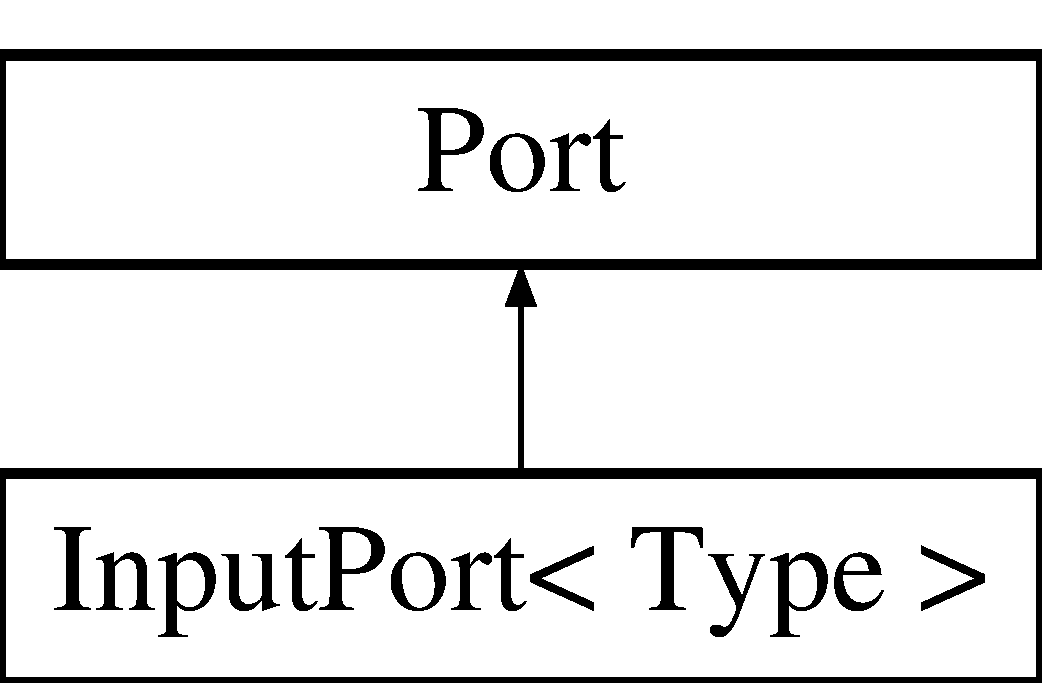
\includegraphics[height=2.000000cm]{classInputPort}
\end{center}
\end{figure}
\subsection*{Public Member Functions}
\begin{DoxyCompactItemize}
\item 
\hyperlink{classInputPort_acf909d66728fd235b335c424d807e91c}{Input\-Port} (string name)
\item 
void \hyperlink{classInputPort_a1a2a37ffa8834ff478ea94458ee34b4f}{consume} (Type $\ast$bn)
\item 
Type $\ast$ \hyperlink{classInputPort_a1022cb16047cf6f8d5510fbdd187333c}{read} ()
\item 
\hyperlink{classInputPort_ab8ca4f0de1d52859f6b69fbe00ec7a71}{$\sim$\-Input\-Port} ()
\end{DoxyCompactItemize}
\subsection*{Additional Inherited Members}


\subsection{Detailed Description}
\subsubsection*{template$<$class Type$>$class Input\-Port$<$ Type $>$}

\hyperlink{classInputPort}{Input\-Port} class is a subclass of the \hyperlink{classPort}{Port} class. It is a class template and the type of the buffer of the port is a template. 

\subsection{Constructor \& Destructor Documentation}
\hypertarget{classInputPort_acf909d66728fd235b335c424d807e91c}{\index{Input\-Port@{Input\-Port}!Input\-Port@{Input\-Port}}
\index{Input\-Port@{Input\-Port}!InputPort@{Input\-Port}}
\subsubsection[{Input\-Port}]{\setlength{\rightskip}{0pt plus 5cm}template$<$class Type $>$ {\bf Input\-Port}$<$ Type $>$\-::{\bf Input\-Port} (
\begin{DoxyParamCaption}
\item[{string}]{name}
\end{DoxyParamCaption}
)\hspace{0.3cm}{\ttfamily [inline]}}}\label{classInputPort_acf909d66728fd235b335c424d807e91c}
\hyperlink{classInputPort}{Input\-Port} constructor


\begin{DoxyParams}{Parameters}
{\em name} & The name of the port \\
\hline
{\em owner} & The owner of the port \\
\hline
\end{DoxyParams}
\hypertarget{classInputPort_ab8ca4f0de1d52859f6b69fbe00ec7a71}{\index{Input\-Port@{Input\-Port}!$\sim$\-Input\-Port@{$\sim$\-Input\-Port}}
\index{$\sim$\-Input\-Port@{$\sim$\-Input\-Port}!InputPort@{Input\-Port}}
\subsubsection[{$\sim$\-Input\-Port}]{\setlength{\rightskip}{0pt plus 5cm}template$<$class Type $>$ {\bf Input\-Port}$<$ Type $>$\-::$\sim${\bf Input\-Port} (
\begin{DoxyParamCaption}
{}
\end{DoxyParamCaption}
)\hspace{0.3cm}{\ttfamily [inline]}}}\label{classInputPort_ab8ca4f0de1d52859f6b69fbe00ec7a71}
\hyperlink{classInputPort}{Input\-Port} destructor 

\subsection{Member Function Documentation}
\hypertarget{classInputPort_a1a2a37ffa8834ff478ea94458ee34b4f}{\index{Input\-Port@{Input\-Port}!consume@{consume}}
\index{consume@{consume}!InputPort@{Input\-Port}}
\subsubsection[{consume}]{\setlength{\rightskip}{0pt plus 5cm}template$<$class Type $>$ void {\bf Input\-Port}$<$ Type $>$\-::consume (
\begin{DoxyParamCaption}
\item[{Type $\ast$}]{bn}
\end{DoxyParamCaption}
)\hspace{0.3cm}{\ttfamily [inline]}}}\label{classInputPort_a1a2a37ffa8834ff478ea94458ee34b4f}
Consume a data coming from The output port calls the consume of input port and owner of this port is executed


\begin{DoxyParams}{Parameters}
{\em bn} & the data to be consumed \\
\hline
\end{DoxyParams}
\hypertarget{classInputPort_a1022cb16047cf6f8d5510fbdd187333c}{\index{Input\-Port@{Input\-Port}!read@{read}}
\index{read@{read}!InputPort@{Input\-Port}}
\subsubsection[{read}]{\setlength{\rightskip}{0pt plus 5cm}template$<$class Type $>$ Type$\ast$ {\bf Input\-Port}$<$ Type $>$\-::read (
\begin{DoxyParamCaption}
{}
\end{DoxyParamCaption}
)\hspace{0.3cm}{\ttfamily [inline]}}}\label{classInputPort_a1022cb16047cf6f8d5510fbdd187333c}
Read data from the port

\begin{DoxyReturn}{Returns}
input buffer of the port 
\end{DoxyReturn}


The documentation for this class was generated from the following file\-:\begin{DoxyCompactItemize}
\item 
core/Port.\-h\end{DoxyCompactItemize}

\hypertarget{classMessage}{\section{Message Class Reference}
\label{classMessage}\index{Message@{Message}}
}


{\ttfamily \#include $<$Message.\-h$>$}

\subsection*{Public Member Functions}
\begin{DoxyCompactItemize}
\item 
void \hyperlink{classMessage_a11b6668bc87e2768d4f4049796a1c8c8}{set\-Prop} (const string \&key, const string \&val)
\item 
Message\-Error \hyperlink{classMessage_a13afe897a221adcd40f5d79cfd6ca2c9}{get\-Prop\-Int} (const string \&key, int \&val)
\item 
Message\-Error \hyperlink{classMessage_a7f96d564782e4c2fdccdd92f3c73d617}{get\-Prop\-String} (const string \&key, string \&val)
\item 
void \hyperlink{classMessage_af57b11eb741f83481ab73387f1d595bb}{set\-Prop\-Int} (const string \&key, const int \&val)
\end{DoxyCompactItemize}


\subsection{Detailed Description}
\hyperlink{classMessage}{Message} to communicate between the filters. 

\subsection{Member Function Documentation}
\hypertarget{classMessage_a13afe897a221adcd40f5d79cfd6ca2c9}{\index{Message@{Message}!get\-Prop\-Int@{get\-Prop\-Int}}
\index{get\-Prop\-Int@{get\-Prop\-Int}!Message@{Message}}
\subsubsection[{get\-Prop\-Int}]{\setlength{\rightskip}{0pt plus 5cm}Message\-Error Message\-::get\-Prop\-Int (
\begin{DoxyParamCaption}
\item[{const string \&}]{key, }
\item[{int \&}]{val}
\end{DoxyParamCaption}
)\hspace{0.3cm}{\ttfamily [inline]}}}\label{classMessage_a13afe897a221adcd40f5d79cfd6ca2c9}
Get the integer message by passing the key


\begin{DoxyParams}{Parameters}
{\em key} & the key of the message \\
\hline
{\em val} & reference to receive the value of the message\\
\hline
\end{DoxyParams}
\begin{DoxyReturn}{Returns}
M\-S\-G\-\_\-\-O\-K if the message is found and M\-S\-G\-\_\-\-N\-O\-T\-\_\-\-F\-O\-U\-N\-D if the message is not found. 
\end{DoxyReturn}
\hypertarget{classMessage_a7f96d564782e4c2fdccdd92f3c73d617}{\index{Message@{Message}!get\-Prop\-String@{get\-Prop\-String}}
\index{get\-Prop\-String@{get\-Prop\-String}!Message@{Message}}
\subsubsection[{get\-Prop\-String}]{\setlength{\rightskip}{0pt plus 5cm}Message\-Error Message\-::get\-Prop\-String (
\begin{DoxyParamCaption}
\item[{const string \&}]{key, }
\item[{string \&}]{val}
\end{DoxyParamCaption}
)\hspace{0.3cm}{\ttfamily [inline]}}}\label{classMessage_a7f96d564782e4c2fdccdd92f3c73d617}
Get the string message by passing the key


\begin{DoxyParams}{Parameters}
{\em key} & the key of the message \\
\hline
{\em val} & reference to receive the value of the message\\
\hline
\end{DoxyParams}
\begin{DoxyReturn}{Returns}
M\-S\-G\-\_\-\-O\-K if the message is found and M\-S\-G\-\_\-\-N\-O\-T\-\_\-\-F\-O\-U\-N\-D if the message is not found. 
\end{DoxyReturn}
\hypertarget{classMessage_a11b6668bc87e2768d4f4049796a1c8c8}{\index{Message@{Message}!set\-Prop@{set\-Prop}}
\index{set\-Prop@{set\-Prop}!Message@{Message}}
\subsubsection[{set\-Prop}]{\setlength{\rightskip}{0pt plus 5cm}void Message\-::set\-Prop (
\begin{DoxyParamCaption}
\item[{const string \&}]{key, }
\item[{const string \&}]{val}
\end{DoxyParamCaption}
)\hspace{0.3cm}{\ttfamily [inline]}}}\label{classMessage_a11b6668bc87e2768d4f4049796a1c8c8}
Set the string message by key and value


\begin{DoxyParams}{Parameters}
{\em key} & the key of the message \\
\hline
{\em val} & the string value of the message \\
\hline
\end{DoxyParams}
\hypertarget{classMessage_af57b11eb741f83481ab73387f1d595bb}{\index{Message@{Message}!set\-Prop\-Int@{set\-Prop\-Int}}
\index{set\-Prop\-Int@{set\-Prop\-Int}!Message@{Message}}
\subsubsection[{set\-Prop\-Int}]{\setlength{\rightskip}{0pt plus 5cm}void Message\-::set\-Prop\-Int (
\begin{DoxyParamCaption}
\item[{const string \&}]{key, }
\item[{const int \&}]{val}
\end{DoxyParamCaption}
)\hspace{0.3cm}{\ttfamily [inline]}}}\label{classMessage_af57b11eb741f83481ab73387f1d595bb}
Set the integer message by key and value


\begin{DoxyParams}{Parameters}
{\em key} & the key of the message \\
\hline
{\em val} & the integer value of the message \\
\hline
\end{DoxyParams}


The documentation for this class was generated from the following file\-:\begin{DoxyCompactItemize}
\item 
core/Message.\-h\end{DoxyCompactItemize}

\hypertarget{classOutputPort}{\section{Output\-Port$<$ Type $>$ Class Template Reference}
\label{classOutputPort}\index{Output\-Port$<$ Type $>$@{Output\-Port$<$ Type $>$}}
}


{\ttfamily \#include $<$Port.\-h$>$}

Inheritance diagram for Output\-Port$<$ Type $>$\-:\begin{figure}[H]
\begin{center}
\leavevmode
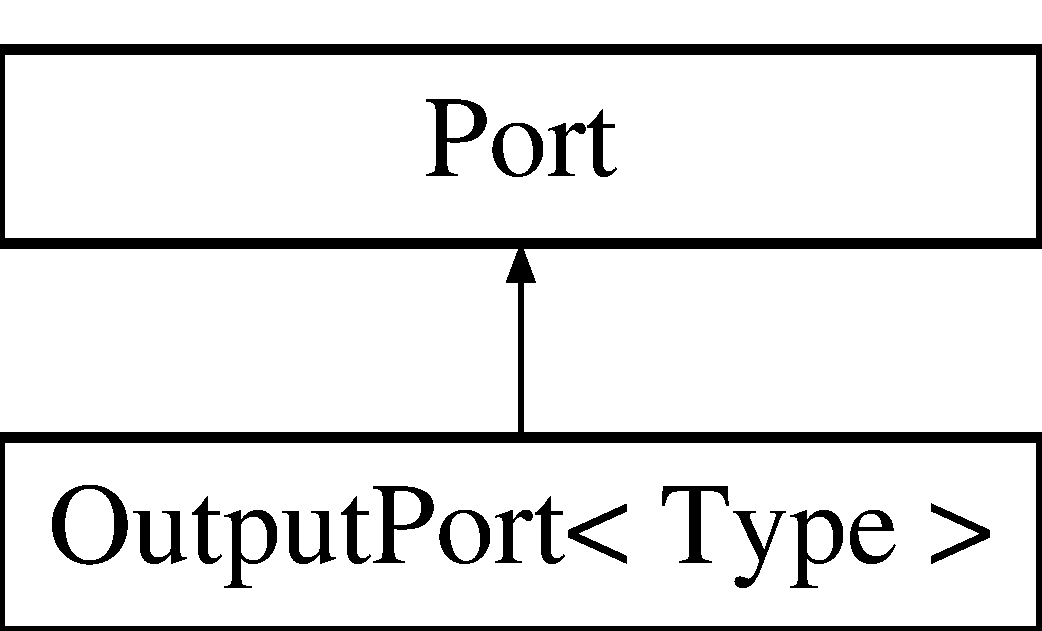
\includegraphics[height=2.000000cm]{classOutputPort}
\end{center}
\end{figure}
\subsection*{Public Member Functions}
\begin{DoxyCompactItemize}
\item 
\hyperlink{classOutputPort_a98259a5fe42207262746c804152ce711}{Output\-Port} (string name)
\item 
void \hyperlink{classOutputPort_a18fe6d7d5be0a04f23b9048124553fa3}{produce} (Type $\ast$bn)
\item 
\hyperlink{classBuffer}{Buffer}$<$ Type $>$ $\ast$ \hyperlink{classOutputPort_a0bd9c526a6d3848fd5ecdcc4935c3f43}{get\-Buffer} ()
\item 
void \hyperlink{classOutputPort_ab6ef20f12eab6ac3188fff5f9bf34074}{process\-Thread} (\hyperlink{classFilter}{Filter} $\ast$f)
\item 
\hypertarget{classOutputPort_a42af5c7e99f82f595386e2c0d21da5ce}{void {\bfseries process} (\hyperlink{classFilter}{Filter} $\ast$f)}\label{classOutputPort_a42af5c7e99f82f595386e2c0d21da5ce}

\item 
\hyperlink{classOutputPort_ac77e96c8a7b605b011043efdc5a905df}{$\sim$\-Output\-Port} ()
\end{DoxyCompactItemize}
\subsection*{Additional Inherited Members}


\subsection{Detailed Description}
\subsubsection*{template$<$class Type$>$class Output\-Port$<$ Type $>$}

\hyperlink{classOutputPort}{Output\-Port} class is a subclass of the \hyperlink{classPort}{Port} class. It is a class template and the type of the buffer of the port is a template. 

\subsection{Constructor \& Destructor Documentation}
\hypertarget{classOutputPort_a98259a5fe42207262746c804152ce711}{\index{Output\-Port@{Output\-Port}!Output\-Port@{Output\-Port}}
\index{Output\-Port@{Output\-Port}!OutputPort@{Output\-Port}}
\subsubsection[{Output\-Port}]{\setlength{\rightskip}{0pt plus 5cm}template$<$class Type $>$ {\bf Output\-Port}$<$ Type $>$\-::{\bf Output\-Port} (
\begin{DoxyParamCaption}
\item[{string}]{name}
\end{DoxyParamCaption}
)\hspace{0.3cm}{\ttfamily [inline]}}}\label{classOutputPort_a98259a5fe42207262746c804152ce711}
\hyperlink{classOutputPort}{Output\-Port} constructor


\begin{DoxyParams}{Parameters}
{\em name} & The name of the output port \\
\hline
{\em owner} & The owner of the port \\
\hline
\end{DoxyParams}
\hypertarget{classOutputPort_ac77e96c8a7b605b011043efdc5a905df}{\index{Output\-Port@{Output\-Port}!$\sim$\-Output\-Port@{$\sim$\-Output\-Port}}
\index{$\sim$\-Output\-Port@{$\sim$\-Output\-Port}!OutputPort@{Output\-Port}}
\subsubsection[{$\sim$\-Output\-Port}]{\setlength{\rightskip}{0pt plus 5cm}template$<$class Type $>$ {\bf Output\-Port}$<$ Type $>$\-::$\sim${\bf Output\-Port} (
\begin{DoxyParamCaption}
{}
\end{DoxyParamCaption}
)\hspace{0.3cm}{\ttfamily [inline]}}}\label{classOutputPort_ac77e96c8a7b605b011043efdc5a905df}
\hyperlink{classOutputPort}{Output\-Port} desctructor 

\subsection{Member Function Documentation}
\hypertarget{classOutputPort_a0bd9c526a6d3848fd5ecdcc4935c3f43}{\index{Output\-Port@{Output\-Port}!get\-Buffer@{get\-Buffer}}
\index{get\-Buffer@{get\-Buffer}!OutputPort@{Output\-Port}}
\subsubsection[{get\-Buffer}]{\setlength{\rightskip}{0pt plus 5cm}template$<$class Type $>$ {\bf Buffer}$<$Type$>$$\ast$ {\bf Output\-Port}$<$ Type $>$\-::get\-Buffer (
\begin{DoxyParamCaption}
{}
\end{DoxyParamCaption}
)\hspace{0.3cm}{\ttfamily [inline]}}}\label{classOutputPort_a0bd9c526a6d3848fd5ecdcc4935c3f43}
Get buffer

\begin{DoxyReturn}{Returns}
the output port buffer 
\end{DoxyReturn}
\hypertarget{classOutputPort_ab6ef20f12eab6ac3188fff5f9bf34074}{\index{Output\-Port@{Output\-Port}!process\-Thread@{process\-Thread}}
\index{process\-Thread@{process\-Thread}!OutputPort@{Output\-Port}}
\subsubsection[{process\-Thread}]{\setlength{\rightskip}{0pt plus 5cm}template$<$class Type $>$ void {\bf Output\-Port}$<$ Type $>$\-::process\-Thread (
\begin{DoxyParamCaption}
\item[{{\bf Filter} $\ast$}]{f}
\end{DoxyParamCaption}
)\hspace{0.3cm}{\ttfamily [inline]}}}\label{classOutputPort_ab6ef20f12eab6ac3188fff5f9bf34074}
Process the port It calls consume function of the next ports and therefore executes the next filters \hypertarget{classOutputPort_a18fe6d7d5be0a04f23b9048124553fa3}{\index{Output\-Port@{Output\-Port}!produce@{produce}}
\index{produce@{produce}!OutputPort@{Output\-Port}}
\subsubsection[{produce}]{\setlength{\rightskip}{0pt plus 5cm}template$<$class Type $>$ void {\bf Output\-Port}$<$ Type $>$\-::produce (
\begin{DoxyParamCaption}
\item[{Type $\ast$}]{bn}
\end{DoxyParamCaption}
)\hspace{0.3cm}{\ttfamily [inline]}}}\label{classOutputPort_a18fe6d7d5be0a04f23b9048124553fa3}
Produce data This function produce data on the output buffer


\begin{DoxyParams}{Parameters}
{\em bn} & data to be produced \\
\hline
\end{DoxyParams}


The documentation for this class was generated from the following file\-:\begin{DoxyCompactItemize}
\item 
core/Port.\-h\end{DoxyCompactItemize}

\hypertarget{classPipeline}{\section{Pipeline Class Reference}
\label{classPipeline}\index{Pipeline@{Pipeline}}
}


{\ttfamily \#include $<$Pipeline.\-h$>$}

\subsection*{Public Member Functions}
\begin{DoxyCompactItemize}
\item 
\hyperlink{classPipeline_a9366c3d29238e354ce23ceabe7bac256}{Pipeline} (const string \&name)
\item 
void \hyperlink{classPipeline_a1d6641e7688b7d20a228a1b43e31271f}{connect\-Filters} (\hyperlink{classFilter}{Filter} $\ast$fi, \hyperlink{classFilter}{Filter} $\ast$fo)
\item 
Pipeline\-Status \hyperlink{classPipeline_aef6b8382fd35a13b06f91f6eb7c810d2}{init} ()
\item 
Pipeline\-Status \hyperlink{classPipeline_a519b34f00a529a0abb106d91396da99b}{run} ()
\item 
\hyperlink{classPipeline_a527044d53a20f851d0579fbf313a2dec}{$\sim$\-Pipeline} ()
\end{DoxyCompactItemize}


\subsection{Detailed Description}
A pipeline, consisting of a number of interconnected filters. Filters have a many-\/to-\/many relation, with directed pipes. Cycles are not allowed. 

\subsection{Constructor \& Destructor Documentation}
\hypertarget{classPipeline_a9366c3d29238e354ce23ceabe7bac256}{\index{Pipeline@{Pipeline}!Pipeline@{Pipeline}}
\index{Pipeline@{Pipeline}!Pipeline@{Pipeline}}
\subsubsection[{Pipeline}]{\setlength{\rightskip}{0pt plus 5cm}Pipeline\-::\-Pipeline (
\begin{DoxyParamCaption}
\item[{const string \&}]{name}
\end{DoxyParamCaption}
)}}\label{classPipeline_a9366c3d29238e354ce23ceabe7bac256}
\hyperlink{classPipeline}{Pipeline} constructor


\begin{DoxyParams}{Parameters}
{\em name} & The name of the pipeline. \\
\hline
\end{DoxyParams}
\hypertarget{classPipeline_a527044d53a20f851d0579fbf313a2dec}{\index{Pipeline@{Pipeline}!$\sim$\-Pipeline@{$\sim$\-Pipeline}}
\index{$\sim$\-Pipeline@{$\sim$\-Pipeline}!Pipeline@{Pipeline}}
\subsubsection[{$\sim$\-Pipeline}]{\setlength{\rightskip}{0pt plus 5cm}Pipeline\-::$\sim$\-Pipeline (
\begin{DoxyParamCaption}
{}
\end{DoxyParamCaption}
)}}\label{classPipeline_a527044d53a20f851d0579fbf313a2dec}
\hyperlink{classPipeline}{Pipeline} destructor 

\subsection{Member Function Documentation}
\hypertarget{classPipeline_a1d6641e7688b7d20a228a1b43e31271f}{\index{Pipeline@{Pipeline}!connect\-Filters@{connect\-Filters}}
\index{connect\-Filters@{connect\-Filters}!Pipeline@{Pipeline}}
\subsubsection[{connect\-Filters}]{\setlength{\rightskip}{0pt plus 5cm}void Pipeline\-::connect\-Filters (
\begin{DoxyParamCaption}
\item[{{\bf Filter} $\ast$}]{fi, }
\item[{{\bf Filter} $\ast$}]{fo}
\end{DoxyParamCaption}
)}}\label{classPipeline_a1d6641e7688b7d20a228a1b43e31271f}
Create a pipe between two filters in the pipeline. These filters should be in the pipeline.


\begin{DoxyParams}{Parameters}
{\em fi} & The source filter for the pipe. \\
\hline
{\em fo} & The target filter for the pipe. \\
\hline
\end{DoxyParams}
\hypertarget{classPipeline_aef6b8382fd35a13b06f91f6eb7c810d2}{\index{Pipeline@{Pipeline}!init@{init}}
\index{init@{init}!Pipeline@{Pipeline}}
\subsubsection[{init}]{\setlength{\rightskip}{0pt plus 5cm}Pipeline\-Status Pipeline\-::init (
\begin{DoxyParamCaption}
{}
\end{DoxyParamCaption}
)}}\label{classPipeline_aef6b8382fd35a13b06f91f6eb7c810d2}
Initialize the pipeline.

\begin{DoxyReturn}{Returns}
the current pipeline status. 
\end{DoxyReturn}
\hypertarget{classPipeline_a519b34f00a529a0abb106d91396da99b}{\index{Pipeline@{Pipeline}!run@{run}}
\index{run@{run}!Pipeline@{Pipeline}}
\subsubsection[{run}]{\setlength{\rightskip}{0pt plus 5cm}Pipeline\-Status Pipeline\-::run (
\begin{DoxyParamCaption}
{}
\end{DoxyParamCaption}
)}}\label{classPipeline_a519b34f00a529a0abb106d91396da99b}
Run one iteration of the pipeline.

\begin{DoxyReturn}{Returns}
the current pipeline status. 
\end{DoxyReturn}


The documentation for this class was generated from the following files\-:\begin{DoxyCompactItemize}
\item 
core/Pipeline.\-h\item 
core/Pipeline.\-cpp\end{DoxyCompactItemize}

\hypertarget{classPort}{\section{Port Class Reference}
\label{classPort}\index{Port@{Port}}
}


{\ttfamily \#include $<$Port.\-h$>$}

Inheritance diagram for Port\-:\begin{figure}[H]
\begin{center}
\leavevmode
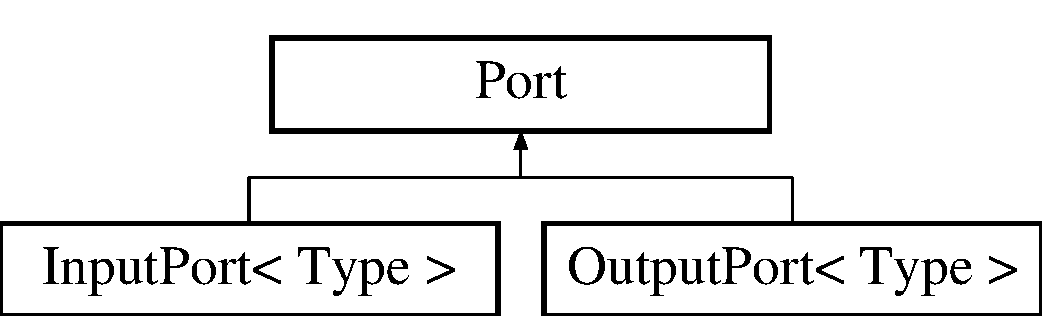
\includegraphics[height=2.000000cm]{classPort}
\end{center}
\end{figure}
\subsection*{Public Member Functions}
\begin{DoxyCompactItemize}
\item 
\hyperlink{classPort_abfb87277bc422b768ccdabd53b23fb83}{Port} (string name)
\item 
string \hyperlink{classPort_a16e393f7d744d91a7d7f8eb6bd675860}{get\-Name} ()
\item 
int \hyperlink{classPort_a8bcebf2e996d12b8bc57cbf17a44ceed}{get\-Linked} ()
\item 
void \hyperlink{classPort_ab3f05bf2221eff2c073e43c215b9507d}{increase\-Linked} ()
\item 
string \hyperlink{classPort_a9a42f2968f394a57b146e8909349c65e}{get\-Type} ()
\item 
vector$<$ \hyperlink{classPort}{Port} $\ast$ $>$ \& \hyperlink{classPort_a9004fcb7c9568ca55857ca37fc3c5c61}{get\-Next\-Ports} ()
\item 
void \hyperlink{classPort_aa78af70b4c46ed8b7a4ee127d5d46d8d}{add\-Next\-Port} (\hyperlink{classPort}{Port} $\ast$n)
\item 
virtual \hyperlink{classPort_a2a6f52a2c46c5f98a3f557707be45c54}{$\sim$\-Port} ()
\end{DoxyCompactItemize}
\subsection*{Protected Attributes}
\begin{DoxyCompactItemize}
\item 
string \hyperlink{classPort_af6073dc317b75da3997f7214e4bcc936}{type}
\item 
vector$<$ \hyperlink{classPort}{Port} $\ast$ $>$ \hyperlink{classPort_a8fc5c440becfcd3ea02cac7656097de1}{next\-Ports}
\end{DoxyCompactItemize}


\subsection{Detailed Description}
Abstraction of a port in a filter. A port can be either input port of output port. 

\subsection{Constructor \& Destructor Documentation}
\hypertarget{classPort_abfb87277bc422b768ccdabd53b23fb83}{\index{Port@{Port}!Port@{Port}}
\index{Port@{Port}!Port@{Port}}
\subsubsection[{Port}]{\setlength{\rightskip}{0pt plus 5cm}Port\-::\-Port (
\begin{DoxyParamCaption}
\item[{string}]{name}
\end{DoxyParamCaption}
)\hspace{0.3cm}{\ttfamily [inline]}}}\label{classPort_abfb87277bc422b768ccdabd53b23fb83}
\hyperlink{classPort}{Port} constructor


\begin{DoxyParams}{Parameters}
{\em name} & The name of the filter. \\
\hline
{\em owner} & The owner of the filter \\
\hline
\end{DoxyParams}
\hypertarget{classPort_a2a6f52a2c46c5f98a3f557707be45c54}{\index{Port@{Port}!$\sim$\-Port@{$\sim$\-Port}}
\index{$\sim$\-Port@{$\sim$\-Port}!Port@{Port}}
\subsubsection[{$\sim$\-Port}]{\setlength{\rightskip}{0pt plus 5cm}virtual Port\-::$\sim$\-Port (
\begin{DoxyParamCaption}
{}
\end{DoxyParamCaption}
)\hspace{0.3cm}{\ttfamily [inline]}, {\ttfamily [virtual]}}}\label{classPort_a2a6f52a2c46c5f98a3f557707be45c54}
\hyperlink{classPort}{Port} descructor 

\subsection{Member Function Documentation}
\hypertarget{classPort_aa78af70b4c46ed8b7a4ee127d5d46d8d}{\index{Port@{Port}!add\-Next\-Port@{add\-Next\-Port}}
\index{add\-Next\-Port@{add\-Next\-Port}!Port@{Port}}
\subsubsection[{add\-Next\-Port}]{\setlength{\rightskip}{0pt plus 5cm}void Port\-::add\-Next\-Port (
\begin{DoxyParamCaption}
\item[{{\bf Port} $\ast$}]{n}
\end{DoxyParamCaption}
)\hspace{0.3cm}{\ttfamily [inline]}}}\label{classPort_aa78af70b4c46ed8b7a4ee127d5d46d8d}
Add next port to this port


\begin{DoxyParams}{Parameters}
{\em n} & next port to connect to \\
\hline
\end{DoxyParams}
\hypertarget{classPort_a8bcebf2e996d12b8bc57cbf17a44ceed}{\index{Port@{Port}!get\-Linked@{get\-Linked}}
\index{get\-Linked@{get\-Linked}!Port@{Port}}
\subsubsection[{get\-Linked}]{\setlength{\rightskip}{0pt plus 5cm}int Port\-::get\-Linked (
\begin{DoxyParamCaption}
{}
\end{DoxyParamCaption}
)\hspace{0.3cm}{\ttfamily [inline]}}}\label{classPort_a8bcebf2e996d12b8bc57cbf17a44ceed}
Get the number of the ports connected to this port

\begin{DoxyReturn}{Returns}
the number of the port. 
\end{DoxyReturn}
\hypertarget{classPort_a16e393f7d744d91a7d7f8eb6bd675860}{\index{Port@{Port}!get\-Name@{get\-Name}}
\index{get\-Name@{get\-Name}!Port@{Port}}
\subsubsection[{get\-Name}]{\setlength{\rightskip}{0pt plus 5cm}string Port\-::get\-Name (
\begin{DoxyParamCaption}
{}
\end{DoxyParamCaption}
)\hspace{0.3cm}{\ttfamily [inline]}}}\label{classPort_a16e393f7d744d91a7d7f8eb6bd675860}
Get the name of the port

\begin{DoxyReturn}{Returns}
the name of the port. 
\end{DoxyReturn}
\hypertarget{classPort_a9004fcb7c9568ca55857ca37fc3c5c61}{\index{Port@{Port}!get\-Next\-Ports@{get\-Next\-Ports}}
\index{get\-Next\-Ports@{get\-Next\-Ports}!Port@{Port}}
\subsubsection[{get\-Next\-Ports}]{\setlength{\rightskip}{0pt plus 5cm}vector$<${\bf Port}$\ast$$>$\& Port\-::get\-Next\-Ports (
\begin{DoxyParamCaption}
{}
\end{DoxyParamCaption}
)\hspace{0.3cm}{\ttfamily [inline]}}}\label{classPort_a9004fcb7c9568ca55857ca37fc3c5c61}
Get the owner of the port

\begin{DoxyReturn}{Returns}
the owner of the filter
\end{DoxyReturn}
Get next ports

\begin{DoxyReturn}{Returns}
the next ports 
\end{DoxyReturn}
\hypertarget{classPort_a9a42f2968f394a57b146e8909349c65e}{\index{Port@{Port}!get\-Type@{get\-Type}}
\index{get\-Type@{get\-Type}!Port@{Port}}
\subsubsection[{get\-Type}]{\setlength{\rightskip}{0pt plus 5cm}string Port\-::get\-Type (
\begin{DoxyParamCaption}
{}
\end{DoxyParamCaption}
)\hspace{0.3cm}{\ttfamily [inline]}}}\label{classPort_a9a42f2968f394a57b146e8909349c65e}
Get the type of the port

\begin{DoxyReturn}{Returns}
the type of the port 
\end{DoxyReturn}
\hypertarget{classPort_ab3f05bf2221eff2c073e43c215b9507d}{\index{Port@{Port}!increase\-Linked@{increase\-Linked}}
\index{increase\-Linked@{increase\-Linked}!Port@{Port}}
\subsubsection[{increase\-Linked}]{\setlength{\rightskip}{0pt plus 5cm}void Port\-::increase\-Linked (
\begin{DoxyParamCaption}
{}
\end{DoxyParamCaption}
)\hspace{0.3cm}{\ttfamily [inline]}}}\label{classPort_ab3f05bf2221eff2c073e43c215b9507d}
Increase the number of the ports linked to the port. (The filter uses this function when it connects two filters) 

\subsection{Member Data Documentation}
\hypertarget{classPort_a8fc5c440becfcd3ea02cac7656097de1}{\index{Port@{Port}!next\-Ports@{next\-Ports}}
\index{next\-Ports@{next\-Ports}!Port@{Port}}
\subsubsection[{next\-Ports}]{\setlength{\rightskip}{0pt plus 5cm}vector$<${\bf Port}$\ast$$>$ Port\-::next\-Ports\hspace{0.3cm}{\ttfamily [protected]}}}\label{classPort_a8fc5c440becfcd3ea02cac7656097de1}
A list of the next ports. A subclass filter must add its filters to this list \hypertarget{classPort_af6073dc317b75da3997f7214e4bcc936}{\index{Port@{Port}!type@{type}}
\index{type@{type}!Port@{Port}}
\subsubsection[{type}]{\setlength{\rightskip}{0pt plus 5cm}string Port\-::type\hspace{0.3cm}{\ttfamily [protected]}}}\label{classPort_af6073dc317b75da3997f7214e4bcc936}
The type of the buffer of the port (note\-: the typeid is used to retrieve the type of the buffer and the type name is not complete. This is used when a filter wants to connect ports and needs to know the type of the ports) 

The documentation for this class was generated from the following file\-:\begin{DoxyCompactItemize}
\item 
core/Port.\-h\end{DoxyCompactItemize}

%--- End generated contents ---

% Index
\newpage
\phantomsection
\addcontentsline{toc}{chapter}{Index}
\printindex

\end{document}
